\documentclass[12pt]{report}
\usepackage[utf8]{inputenc}
\usepackage[margin=1in]{geometry}
\usepackage{titling}
\usepackage[indentafter]{titlesec}
\usepackage[pdfusetitle]{hyperref}
\usepackage[acronym]{glossaries}
\usepackage{enumitem}
\usepackage[numbers]{natbib}
\usepackage{tikz}


% Document Information
\author{Patrick McNamee}
\title{EECS 753 Project Proposal}
\date{\today}


% Hyperref Setup
\hypersetup{
	linkbordercolor={1 1 1},  % White border so it doesn't show
}


% Heading manipulations
\titleclass{\chapter}{straight}
\titlespacing{\chapter}{0in}{10pt}{5pt}
\titleformat{\chapter}[hang]
	{\bfseries\large} % Format
	{} % Label
	{0pt} % Sep
	{} % Before code
	[] % After code


% Acronyms
\newacronym{cnn}{CNN}{convolutional neural network}
\newacronym{gnc}{GNC}{guidance, navigation, and control}
\newacronym{nn}{NN}{neural network}


% Quick Acronym Reference
\newcommand{\CNN}{\acrshort{cnn}}
\newcommand{\GNC}{\acrshort{gnc}}
\newcommand{\NN}{\acrshort{nn}}


\begin{document}
% Title "Page"
\begin{center}
{\Large\bfseries\thetitle}\\
\theauthor\\
\thedate
\end{center}

\chapter{Problem Statement}

As the sector of autonomous vehicles mature, \acrfull{nn} are becoming more prevalent in autonomous vehicles as a means to simplify and accelerate traditional algorithms used for vehicle \acrfull{gnc}. However, unlike the traditional algorithms, \NN\ have no output smoothness guarantee so small perturbations in the network input can lead to drastically different outputs which can often lead to high jerk control inputs.

\chapter{Motivation}

As \acrlong{nn}s are universal approximators with the proofs of such generally using the network architecture and properties of the activation functions \cite{wang2021interval}, they are often candidates to replace other algorithms when speed is critical. Various works show the prevalence of \NN\ within various autonomous cars \cite{bechtel2018, pujol2019, kato2018} although \NN\ are often not used to replace the entire logical chain from environmental perception to control as in \cite{bechtel2018}. However, when \NN s replace the entire logical train, the vehicle can be unsafe and crash whereas the \NN\ that only replace guidance and/or navigation in the vehicle \GNC\ yield safer behavior. Previous work has used \NN s to output B\'ezier curves for smooth navigation curves with an underlying pursuit curve controller for autonomous racing \cite{trent2020iros} but this relies on the vehicle having spatial information either through simultaneous localization and mapping or global positioning systems. Small indoor autonomous vehicles may not have the computational resources or sensors for real-time \GNC\ but the vehicles may be able to utilize the combination of \CNN\ and B\'ezier curves to schedule smooth control commands from vision and outperform platforms using \CNN\ purely to generate commands from vision.

\chapter{Proposed Solution}

The DeepPicar is a remote control model car that has been built to drive around a marked track using a \acrfull{cnn} hosted on a Raspberry Pi \cite{bechtel2018}. While it originally used a \CNN\ to generate steering angle control commands, this project would use a \CNN\ on DeepPicar as a control scheduler using B\'ezier curves to generate smooth steering angle commands. This change in the utilization would allow for smooth control outputs and potentially computational resource saved as the B\'ezier \CNN\ may be able to run at a lower rate than the original \CNN\ while still allowing for real-time \GNC .

\chapter{Project Outline}

This project can be broken down into three parts over the month of April starting April 5, 2021:

\begin{enumerate}[label=Part \arabic*), leftmargin=16ex]
\item Train \CNN\ based data original to the DeepPicar \citep{bechtel2018} or a similiar data set. Weeks 1-3.
\item Implement the real-time controller for DeepPi car where a real-time task \acrfull{cnn} schedules the command steering angle for some time window and an inner loop real-time controller implements the steering angle schedule. Week 2-3.
\item Run experiment to determine performance. Of particular note is the accuracy of the DeepPicar following a racetrack as well as the computational resource cost of this overall control scheme compare to the \CNN\ used in Ref \citep{bechtel2018}. Week 3-4.
\end{enumerate}

\begin{figure}[htb]
\begin{center}
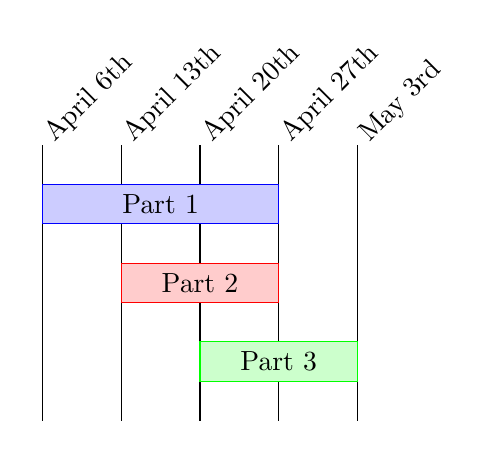
\begin{tikzpicture}

\foreach \x/\date in {0/April 6th, 1/April 13th, 2/April 20th, 3/April 27th, 4/May 3rd}
	{\draw (\x, -0.5) -- (\x,3) node[anchor=west, rotate=45]{\date};}

\filldraw[color=blue, fill=blue!20] (0,2) rectangle node[black]{Part 1} (3,2.5);
\filldraw[color=red, fill=red!20] (1,1) rectangle node[black]{Part 2} (3,1.5);
\filldraw[color=green, fill=green!20] (2,0) rectangle node[black]{Part 3} (4,0.5);

\end{tikzpicture}
\end{center}
\caption{Timeline Gantt Chart}
\end{figure}

Final outcomes of this project is a trained convolutional neural network outputting a B\'ezier curve for control scheduling and some performance benchmarking to determine the change in resource utilization form the original \CNN\ in \cite{bechtel2018}. Benchmarking of the proposed solution should be performed on the DeepPicar and have quantitative CPU resource effects such as scheduled CPU time and worst-case execution time in addition to qualitative driving performance effects such as how far around the track DeepPicar drives and how many times the car drives outside the track bounds.

\renewcommand{\bibname}{References}
\bibliographystyle{IEEEtranN}
\bibliography{proposal}

\end{document}